\begin{frame}
    \frametitle{Hospital Formulation}

    \vspace*{0.5cm}
    \centering
    \begin{figure}[h]
        \begin{tikzpicture}[>=stealth, scale=0.6] %arrow type
            % the rectangle with vertical rules (Queue 1)
            \draw (0,0) -- ++(2cm,0) -- ++(0,-1.5cm) -- ++(-2cm,0);
            \foreach \i in {1,...,4}
            \draw (2cm-\i*10pt,0) -- +(0,-1.5cm);
            
            % the circle (Queue 1)
            \draw (2.75,-0.75cm) circle [radius=0.75cm];
    
            % the rectangle with vertical rules (Queue 2)
            \draw (5,1.25) -- ++(2cm,0) -- ++(0,-1.5cm) -- ++(-2cm,0);
            \foreach \i in {1,...,4}
            \draw (7cm-\i*10pt,1.25) -- +(0,-1.5cm);
    
            % the circle (Queue 2)
            \draw (7.75,0.5) circle [radius=0.75cm];
    
            % the arrows and labels (Queue 1+2)
            \draw[->] (8.5,0.525) -- +(20pt,0);
            \node[align=center] at (1cm,-2cm) {};
            \node[align=center] at (2.75cm,-2cm) {Parking};
            \node[align=center] at (6cm,-0.75cm) {};
            \node[align=center] at (7.8cm,-0.75cm) {Hospital};
            
            % Ambulance lines
            \draw[<-] (0,-0.75) -- +(-50pt,0) node[left] {\( \lambda^a \)};
            \draw[-] (3.5,-0.75) -- +(20pt,0);
            \draw (4.2, 0.525) -- (4.2, -0.75);

            % Others lines
            \draw (4.2, 1.8) -- +(-169.5pt,0) node[left] {\( \lambda^o \)};
            \draw (4.2, 1.8) -- (4.2, 0.525);
            \draw[->] (4.2, 0.525) -- (5, 0.525);

            %%%%%%%%%%%%%%%%
            %% ANIMATIONS %%
            %%%%%%%%%%%%%%%%

            % Stick-figures
            \only<2,3,4,5,6,7,8,9,10>{
                \node[draw=none] at (7.5,0.75) {\Strichmaxerl[1]};
            }
            \only<3,4,5,6,7,8,9>{
                \node[draw=none] at (8,0.75) {\Strichmaxerl[1]};
            }
            \only<4,5,6>{
                \node[draw=none] at (7.75,0.25) {\Strichmaxerl[1]};
            }
            \only<5,6,7,8>{
                \node[draw=none] at (2.75,-0.75) {\Strichmaxerl[1]};
            }
            % Green arrow for hospital arrival
            \only<2,4>{
                \draw[red, very thick] (4.2, 1.8) -- +(-169.5pt,0) node[left] {\( \lambda^o \)};
                \draw[red, very thick] (4.2, 1.8) -- (4.2, 0.525);
                \draw[->, red, very thick] (4.2, 0.525) -- (5, 0.525);
            }
            % Blue Arrow from Parking to Hospital
            \only<3,8,9>{
                \draw[-, blue, very thick] (3.5,-0.75) -- +(20pt,0);
                \draw[blue, very thick] (4.2, 0.525) -- (4.2, -0.75);
                \draw[->, blue, very thick] (4.2, 0.525) -- (5, 0.525);
            }
            % Blue arrow for Parking Arrival
            \only<3,5,6>{
                \draw[<-, blue, very thick] (0,-0.75) -- +(-50pt,0) node[left] {\( \lambda^a \)};
            }
            % Parking waiting line (1 patient)
            \only<6,7>{
                \draw[blue, very thick] (2cm-10pt,0) -- +(0,-1.5cm);
            }
            % Green arrow Exiting Hospital
            \only<7,8,9,10,11>{
                \draw[->, green, very thick] (8.5,0.525) -- +(20pt,0);   
            }
        \end{tikzpicture}
    \end{figure}


    \begin{figure}
        \begin{tikzpicture}[-, node distance = 0.7cm, auto, every node/.style={scale=0.5}]
            \node[state] (one) {(0,0)};
            \only<1,11>{\node[state, ultra thick] (one) {(0,0)};}

            \node[state, right=of one] (two) {(0,1)};
            \only<2,10>{\node[state, ultra thick, right=of one] (two) {(0,1)};}

            \node[state, right=of two] (three) {(0,2)};
            \only<3,9>{\node[state, ultra thick, right=of two] (three) {(0,2)};}

            \node[state, right=of three] (four) {(0,3)};
            \only<4>{\node[state, ultra thick, right=of three] (four) {(0,3)};}

            \node[state, right=of four] (five) {(0,4)};

            \node[state, below=of three] (three_one) {(1,2)};
            \only<8>{
                \node[state, ultra thick, below=of three] (three_one) {(1,2)};
            }            

            \node[state, below=of three_one] (three_two) {(2,2)};
            \only<7>{\node[state, ultra thick, below=of three_one] (three_two) {(2,2)};
            }

            \node[state, below=of four] (four_one) {(1,3)};
            \only<5>{\node[state, ultra thick, below=of four] (four_one) {(1,3)};}

            \node[state, below=of four_one] (four_two) {(2,3)};
            \only<6>{\node[state, ultra thick, below=of four_one] (four_two) {(2,3)};}

            \node[state, below=of five] (five_one) {(1,4)};
            \node[state, below=of five_one] (five_two) {(2,4)};

            \draw[every loop]

                (one) edge[bend left] node {\( \Lambda \)} (two)
                (two) edge[bend left] node {\( \mu \)} (one)
                (two) edge[bend left] node {\( \Lambda \)} (three)
                (three) edge[bend left] node {\( 2\mu \)} (two)
                (three) edge[bend left] node {\( \lambda^o \)} (four)
                (four) edge[bend left] node {\( 3\mu \)} (three)
                (four) edge[bend left] node {\( \lambda^o \)} (five)
                (five) edge[bend left] node {\( 3\mu \)} (four)
                (three) edge[bend left] node {\( \lambda^A \)} (three_one)
                (three_one) edge[bend left] node {\( 2\mu \)} (three)
                (three_one) edge[bend left] node {\( \lambda^o \)} (four_one)
                (four_one) edge[bend left] node {\( 3\mu \)} (three_one)
                (four_one) edge[bend left] node {\( \lambda^o \)} (five_one)
                (five_one) edge[bend left] node {\( 3\mu \)} (four_one)
                (four) edge node {\( \lambda^A \)} (four_one)
                (five) edge node {\( \lambda^A \)} (five_one)
                (three_one) edge[bend left] node {\( \lambda^A \)} (three_two)
                (three_two) edge[bend left] node {\( 2\mu \)} (three_one)
                (four_one) edge node {\( \lambda^A \)} (four_two)
                (five_one) edge node {\( \lambda^A \)} (five_two)
                (three_two) edge[bend left] node {\( \lambda^o \)} (four_two)
                (four_two) edge[bend left] node {\( 3\mu \)} (three_two)
                (four_two) edge[bend left] node {\( \lambda^o \)} (five_two)
                (five_two) edge[bend left] node {\( 3\mu \)} (four_two)
                ;       
        \end{tikzpicture}
        \caption*{C=3, T=2, N=4, M=2}
    \end{figure}
\end{frame}